%\documentclass[12pt]{article}
\documentclass[12pt]{extarticle}
\usepackage[utf8]{inputenc}
\usepackage[margin=0.5in]{geometry}
\usepackage{enumitem}
\usepackage{graphicx}
\usepackage{float}
\usepackage{romannum}
 
 % Title page
\title{VAST 2019 Weekly Report 2}
\author{Vivek Koodli Udupa}
\date{\today}

\begin{document}
\pagenumbering{arabic}
\maketitle

% INTRODUCTION
\begin{centering}
	\section{Introduction}
\end{centering}
This report will address the credibility of the damages reported by the citizens of St. Himark using the RUMBLE app. As addressed in Report 1, the number of damage reports coming in from different locations are unbalanced. Some locations have high number of reports where as some locations have very few entries. This report addresses ways to deal with this nonuniform distribution of data and analyzing the reliability of damages reported.  \\

% VISUALIZATION	
\begin{centering}
	\section{Visualization and Analysis}
\end{centering}

%Plot of Maps
\begin{figure}[H]
	\centering
	\begin{minipage}{0.5\textwidth}
		\centering
		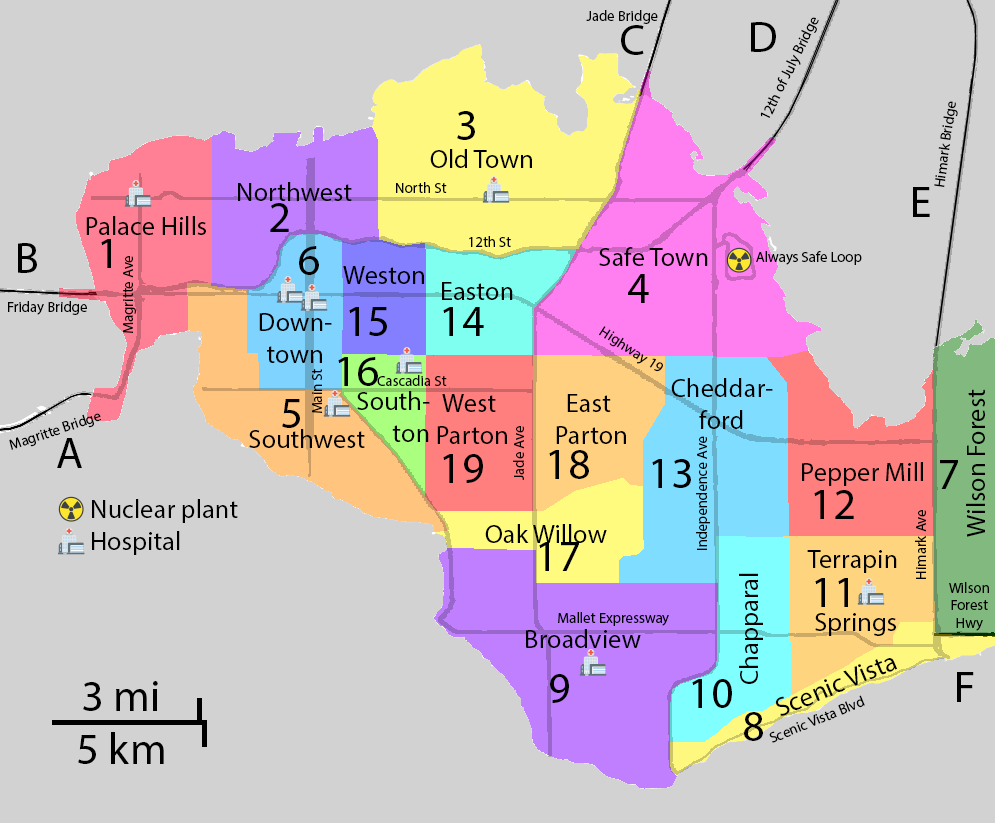
\includegraphics[width=\textwidth]{Images/map.png}
		\caption{St.Himark Neighborhood Map}
		\label{fig:map}
	\end{minipage}%
	\begin{minipage}{0.5\textwidth}
		\centering
		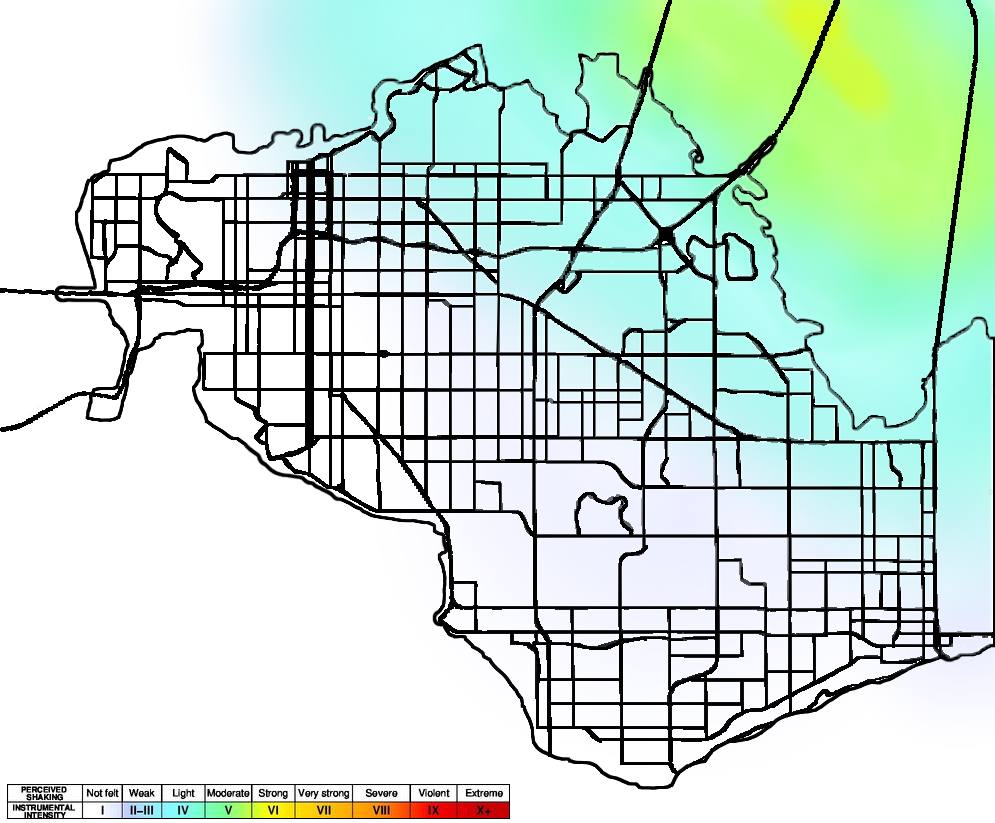
\includegraphics[width=\textwidth]{Images/shakemap.png}
		\caption{St.Himark Shake Map}
		\label{fig:shakemap}
	\end{minipage}
\end{figure} 

% Damage plot
\begin{figure}[H]
\centering
	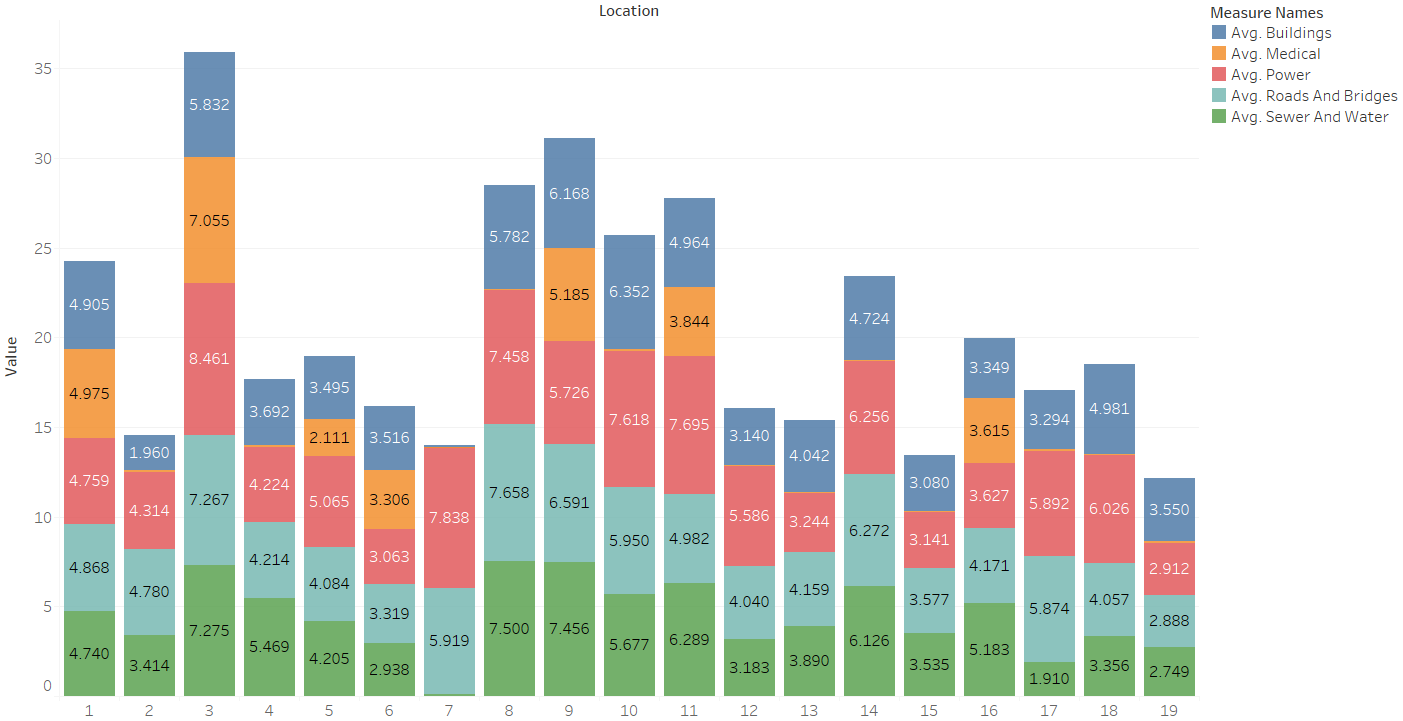
\includegraphics[width=\linewidth]{Images/AllDamage.png}
	\caption{Cumulative damage for different locations }
	\label{fig:alldamage}
\end{figure}

Figure \ref{fig:alldamage} shows the total damage sustained by different locations, which were observed and reported by the citizens of St. Himark. This figure raises suspicion. Locations 1, 8, 9 and 10 shows relatively high damage even though they are not in the earthquake shake zone as shown in Figure \ref{fig:shakemap}. The high damage of Location 3 is acceptable as it resides directly in the shake zone. what could be the cause for the high damage reports in other locations? Are the data collected from RUMBLE reliable? \\

From the description of St. Himark [1] given in the documentation of VAST 2019 MiniChallenge 1, there were several ongoing road and water related repairs taking place before the earthquake disaster. These repairs caused road blocks and possibly inaccessibility to water for the citizens of St. Himark. Thus citizens might have reported damages even before the earthquake took place. \\

To verify this, we must first figure out the date and time the earthquake hit the city. Figures \ref{fig:date} through \ref{fig:timeZoom} tries to visualize the same. \\

Figure \ref{fig:date} shows the shake intensity recorded at different locations on various days.  Figure \ref{fig:dateZoom} is the zoomed in version of Figure \ref{fig:date}, showing only Location 3, making it easier to see the details in the graph. The recorded shake intensity spikes on 8th april 2020.  Next step is to pinpoint the time of earthquake's impact. \\

Figure \ref{fig:time} and Figure \ref{fig:timeZoom} shows the shake intensity recorded at different locations in St. Himark at different time intervals. \\

%Date Plot
\begin{figure}[H]
\centering
	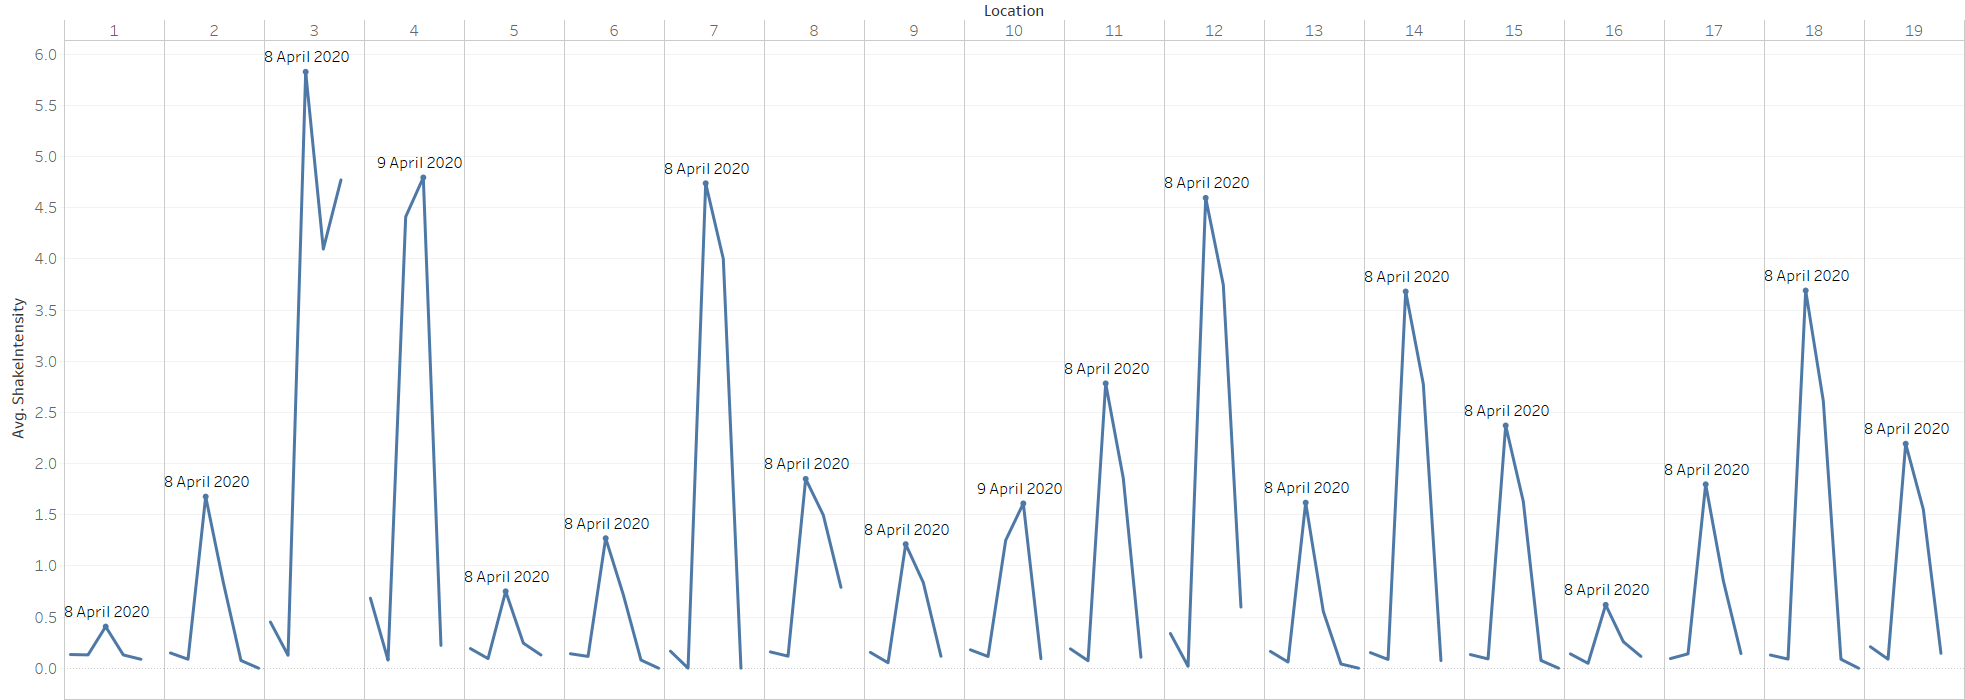
\includegraphics[width=\linewidth]{Images/Date.png}
	\caption{Date vs Shake intensity for all Locations }
	\label{fig:date}
\end{figure}

\begin{figure}[H]
\centering
	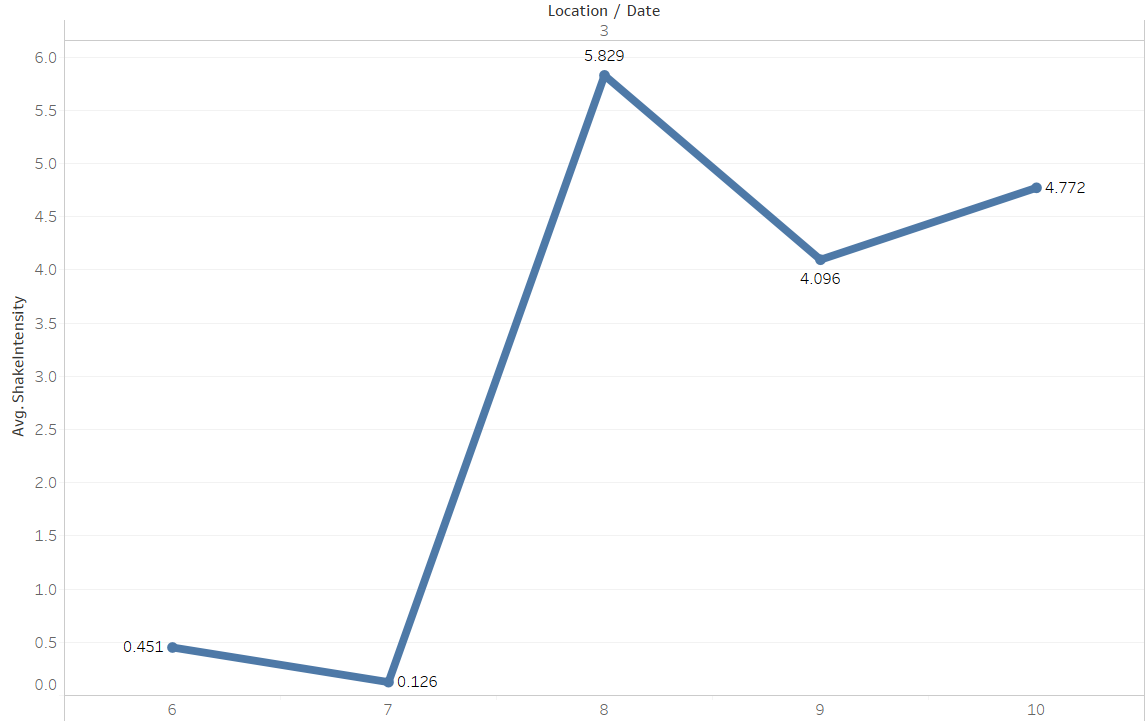
\includegraphics[width=0.5\linewidth]{Images/DateZoom.png}
	\caption{Date vs Shake intensity for Location 3 }
	\label{fig:dateZoom}
\end{figure}

Figure \ref{fig:timeZoom} is just a zoomed into location 3 version of Figure \ref{fig:time}. Purpose of Figure \ref{fig:timeZoom} is to help see the details as Figure \ref{fig:time} is too small to highlight the finer details in the plot.  \\

A prominent pattern that catches the eye while analyzing the plots is that the shake intensity spikes between 8:00 am and 9:00 am consistently in every location. \\ 

Having an idea of the data and time of the earthquake, the damage reports can be split up into before and after the earthquake for more in-dept analysis of the aftermath of the earthquake. \\
%Time plot
\begin{figure}[H]
\centering
	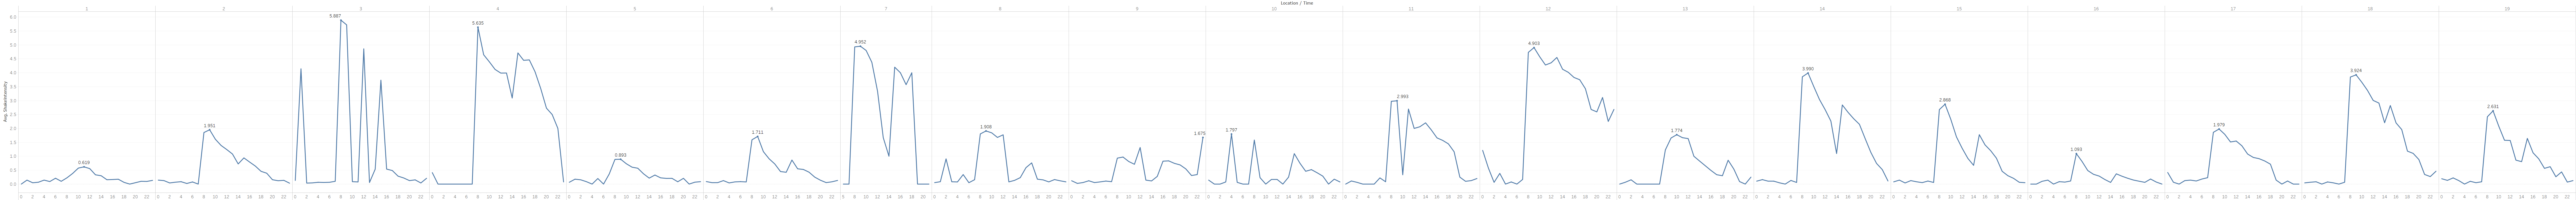
\includegraphics[width=\linewidth]{Images/time.png}
	\caption{Time of Earthquake}
	\label{fig:time}
\end{figure}

\begin{figure}[H]
\centering
	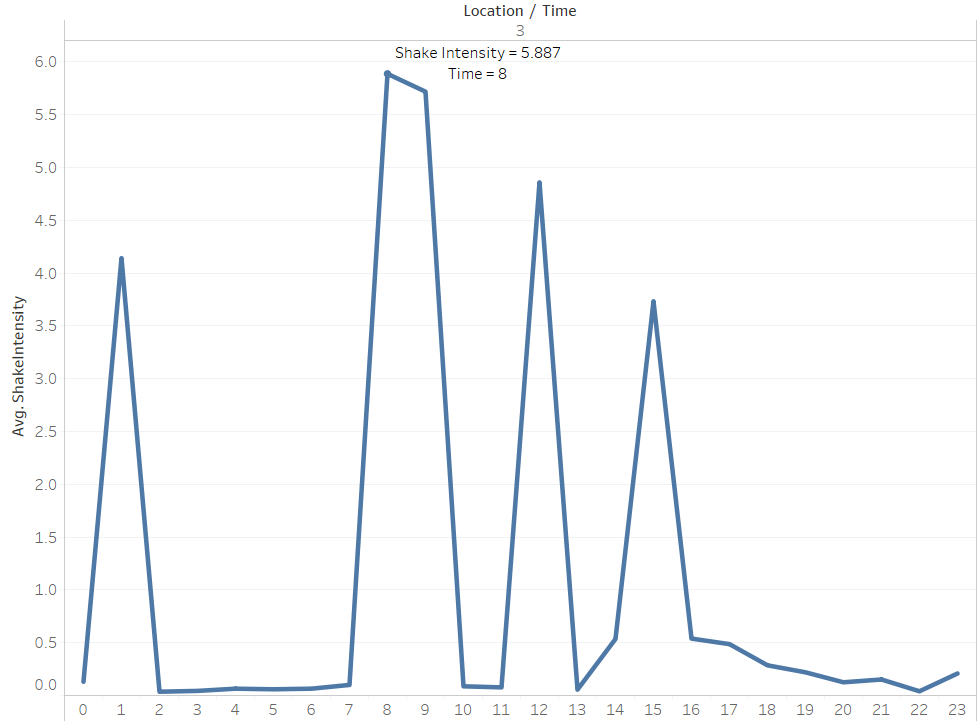
\includegraphics[width=0.5\linewidth]{Images/timeZoom.png}
	\caption{Time of Earthquake Zoomed into Location 3}
	\label{fig:timeZoom}
\end{figure}

Having analyzed the time of impact, the next step further is to find a rationale as to why locations 1, 8, 9 and 10 have high relative damages while being away form the earthquake shake zone. \\

\subsection{Location 1: Palace Hills}
From the description of St. Himark [1], palace hill looks to be a luxurious rich city. It has private beaches and gated communities ensuring fun and safety for the residents. Having only 1662 damage recordings out of the total 83,070, Palace Hill accounts to only 2\% of the entire damages reported. This could be because of low population density. Palace hill seems to be a place for laid back, rich and retired class of citizens. As majority of the working class prefer cheaper residence and shorter commute to work, the population of Palace hill just might be full of people who wants a relaxed, slow paced life. \\

% Mode Plot for Location 1
\begin{figure}[H]
\centering
	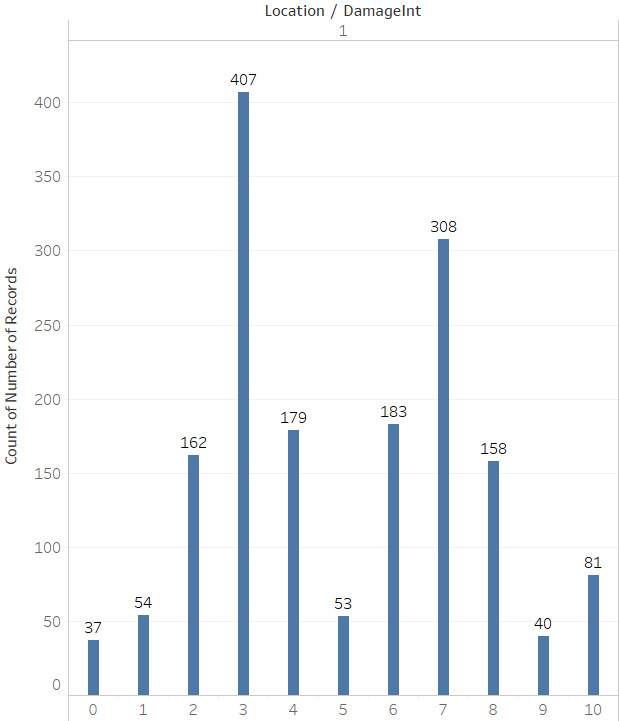
\includegraphics[width=0.4\linewidth]{Images/Loc1Mode.png}
	\caption{Number of Reports for different damage intensity at location 1 }
	\label{fig:mode}
\end{figure}

Having a smaller population means that everyone's damage report weighs more while analyzing the damage. Outliers could cause noticeable changes in the graph shown in Figure \ref{fig:alldamage}. To verify this, Figure \ref{fig:mode} shows the plot of number of reports for different damage intensity recorded for location 1. The X-axis represents the different damage intensities, 0 being the lowest and 10 being the highest. Y-axis marks the number of reports recorded through RUMBLE. \\

Here, it can be observed that the damage 3 and damage 7 are prominent. The cause of this could be that the people close to Northwest(Location Id: 2) might have observed more damage as compared to the people of palace hill living far across the other end of the city.  

\subsection{Location 8: Scenic Vista}
Scenic Vista is described as a trendy, hillside apartments overlooking the ocean, home for the elite of St. Himark [1]. Scenic Vista is well away from the shake zone and has still reported high damages as seen in Figure \ref{fig:alldamage}. There are no records of repairs at Scenic Vista. Thus there is no solid evidence to support the claim of heavy damages in this location.

\subsection{Location 9 and 10: Broadview and Chapparal}
Broadview and Chapparal are both described as old cities with rustic 18th and 19th century buildings [1]. The structural integrity of these buildings could be weak and the small effect of the earthquake might have caused considerable damage to these cities. 

% Conclusion
\begin{centering}
	\section{Conclusion}
\end{centering}

The goal of this report was to test the reliability of the damages recorded on the RUMBLE app. The date and time of the earthquake was found to be April 8, 2020 between 8:00 am and 9:00 am . Figure \ref{fig:date} through Figure \ref{fig:timeZoom} shows clear peaks at the mentioned date and time. Having known the exact time of earthquake, all the damage reports prior to 8:00am of April 8 can be discarded. \\

Few locations had reports of high damage. These reports were suspicious because the locations were far away from the earthquake. \\
The data collected from Palace Hill, location 1 seems to be credible as a portion of the city might have been effected while the rest did not. The smaller population of the city and the possible of concentration of people near the Northern end of the city might have caused the reports to be skewed towards the higher end. Since the location within the city cannot be tracked, there is no way of cross-checking this hypothesis. \\
The data collected from Scenic Vista, location 8 seems to be unreliable. The location is the farthest from the earthquake, there were no recorded repairs and the place is well maintained by the elites of the Community. Thus, the only conclusion for the high damage is that the elites might have reported a higher than actual damage ratings through the app. \\
The damage at location 9 and 10 seems to be caused due to the low structural integrity of the older buildings at Broadview and Chapparal cities. These damage reports can be considered as credible. 



% Reference
\begin{centering}
	\section{Reference}
\end{centering}
[1] VAST 2019 - St. Himark -  About our City.docx

\end{document}


